We performed a series of experiments to test the robustness of the
self-stabilizing algorithms in the sec{[}x{]}. We focus on evaluating
overhead and convergence property in presence of soft faults. 

While there is not much different in applying self-stabilization to
Async and Sync vriants, we focus only on Async case here. Async case
is considerably more difficult than Sync case, as in Async case a
single fault can propagate to multiple vertices in a single iteration.
Moreover, Async case keeps only a single copy of the state, so self-correction
approach taht works well on Sync case, will not work on Async case\footnote{We compared the self-correcting and the self-stabilizing algorithm
for Sync algorithm, and self-correcting label propagation performs
definitively better.}.

\begin{comment}
\textbf{\emph{p}}\emph{urpose of this section} 
\begin{itemize}
\item what do we want to show 
\item why do we want to show 
\item how do we want to show 
\end{itemize}

\paragraph{\emph{experimental setup} }
\begin{itemize}
\item system description 
\item programming environment 
\item test matrices 
\end{itemize}
\end{comment}


\subsection{Experimental set-up}

\subsubsection{Test-bed}

We prototyped our implementation in C and compiled with Intel C compiler
(insert compiler version) with $O3$ optimization flages. We ran our
experiments in a dual socket Ivy-bridge with $2\times8$cores running
at 2.66GHz. This testbed had 128GB DRAM and 12Mb of L3.

\subsubsection{Test-networks}

We choose networks from real applications with diverse sparsity pattern,
density, degree distribution and component distribution. In table{[}x{]},
we list the networks along with some properties.

\begin{table}
\caption{List of the matrices}

%% LyX 2.2.2 created this file.  For more info, see http://www.lyx.org/.
%% Do not edit unless you really know what you are doing.
\documentclass[english]{article}
\usepackage[T1]{fontenc}
\usepackage[latin9]{inputenc}

\makeatletter

%%%%%%%%%%%%%%%%%%%%%%%%%%%%%% LyX specific LaTeX commands.
%% Because html converters don't know tabularnewline
\providecommand{\tabularnewline}{\\}

\makeatother

\usepackage{babel}
\begin{document}
\begin{table*}[t]
\caption{List of the matrices}

\begin{tabular}{|c|c|c|c|}
\hline 
Name & Source & $\left(V\right)$ & $\frac{V}{E}$\tabularnewline
\hline 
\hline 
Kron\_simple\_500 log 18 & Random Kronecker Graph & 262,144  & 21,165,908\tabularnewline
\hline 
rgg(2,18) &  & 262,144 & 3,094,566\tabularnewline
\hline 
astro-ph &  & 16706 & 242502\tabularnewline
\hline 
cond-mat &  & 16726 & 95188\tabularnewline
\hline 
cond-mat-2005 &  & 40421 & 351382\tabularnewline
\hline 
caidaRouterLevel &  & 192244 & 1218132\tabularnewline
\hline 
Kron\_(500,18) &  & 262,144  & 21,165,908\tabularnewline
\hline 
polblogs &  & 1490 & 19025\tabularnewline
\hline 
Wordnet3 &  & 82,670 & 132,964\tabularnewline
\hline 
patents\_main &  & 240,547  & 560,943\tabularnewline
\hline 
email\_EuAll &  & 265,214  & 420,045\tabularnewline
\hline 
soc-sign-epinions &  & 131,828 & 841,372\tabularnewline
\hline 
web-Google &  & 916,428 & 5,105,039\tabularnewline
\hline 
web-Stanford &  & 281,903 & 2,312,497\tabularnewline
\hline 
cit-HepTh &  & 27,770  & 352,807 \tabularnewline
\hline 
webbae-1M &  & 1000005 & 3105536\tabularnewline
\hline 
\end{tabular}
\end{table*}

\end{document}

\end{table}


\subsubsection{Fault injection methodology}

We inject bitflips in memory operation to simulate faults.Specifically,
we inject bitflips in two main memory operation: a) reading adjacency
tree, and b) reading labels of neighbours. Bitflip in an array-index
value may cause memory segmentation error and abort. Therefore, we
gaurd susceptible array-index variable with a range check. If the
variable is out of range, we change it to random value within range.

\subsubsection{Competing algorithms}

In our experiments, we compare the following representative fault
tolerant algorithms:
\begin{enumerate}
\item Baseline: Algm(x) 
\item TMR: Triple modular redundancy 
\item SsLP: Self-stabilizing LP iteration without any checks. 
\item HSsLP: Self-stabilizing LP iteration with unreliable checks. 
\end{enumerate}
%

\subsection{Failure Test}

The aim of failure test is to quantify the frequency of the event
when an algorithm fails to give the correct results, indepedent of
any incurred overhead. This is done by executing each algorithm multiple
times for a given network in simulated random fault environment with
different seeds for random number generation. We compare the four
algorithms based on the success rate at a specific fault rate. The
fault rate is chosen from $\{2^{-5},2^{-6},\ldots2^{-20}\}$ bitflips
per memory operation at which TMR fails for roughly 50\% of the trials. 

Note that SS SSH LP algorithm will almost always give correct results
if we do not limit number of iterations to converge. However, this
doesn't reflect the practical use of the algorithm. Thus, in our experiments
we limit the number of iteration to 100. If an algorithm doesn't converge
by 100 iteration, it aborts and reports failure. 

\begin{figure}
\includegraphics[width=0.9\columnwidth]{plots/failureTest_async_first_0\lyxdot 50}\caption{Success rate for different different test networks }

\end{figure}

In fig(x), we show the success rate of different algorithm for different
graphs at TMR50. Note that this fault inject rate so high that traditional
redundancy based fault tolerance algorithm will fail in \textasciitilde{}50\%
of the cases. In fig(x), we see that SShSv has a success rate of more
than 90\% in 9 out of eleone cases. SShSv is better than TMR in 8
out of 11 cases. 

There are two graphs kron\_g and mouse\_gene where all the algorithm
have very good success rate. This is typically the case when the graph
is relatively dense. RGG is one random graph where Baseline and TMR
have 100\% success rate but both SsSv and SShSV performs extremely
poorly. This usually happens when a graph has a lot of tree like structure.
In such cases even though sssv and sshsv have converged to correct
solution, they may still find a 2-loop 

\subsection{Convergence Test}

\begin{figure*}
\subfloat[Histogram of iteration distribution]{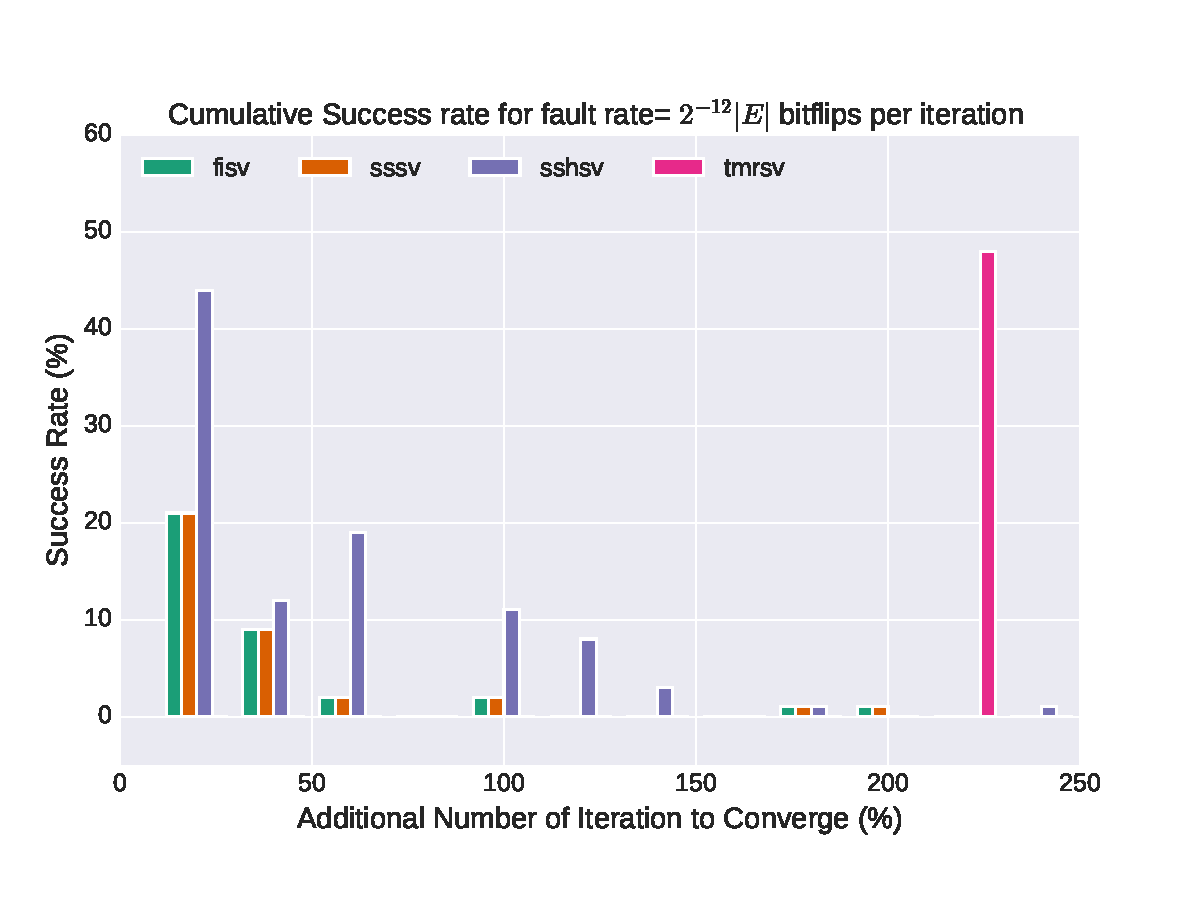
\includegraphics[width=0.4\paperwidth]{plots/astro-ph_async_12_hist}

}\hfill{}\subfloat[Cumulative success rate with respect to addition iteration to converge]{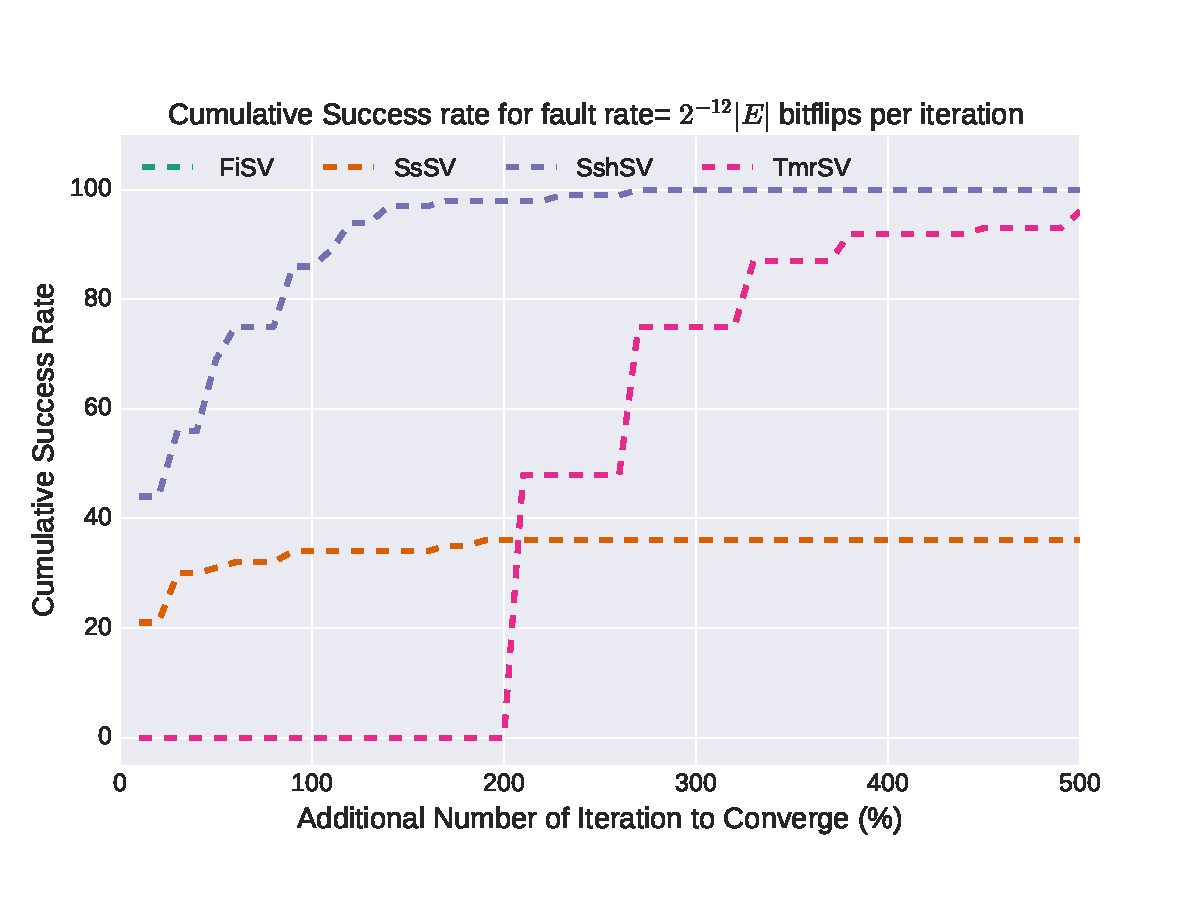
\includegraphics[width=0.4\paperwidth]{plots/astro-ph_async_12_line}}

\caption{Success rate for different different test networks }
\end{figure*}


\subsection{Overhead of Correction step}

\begin{figure}
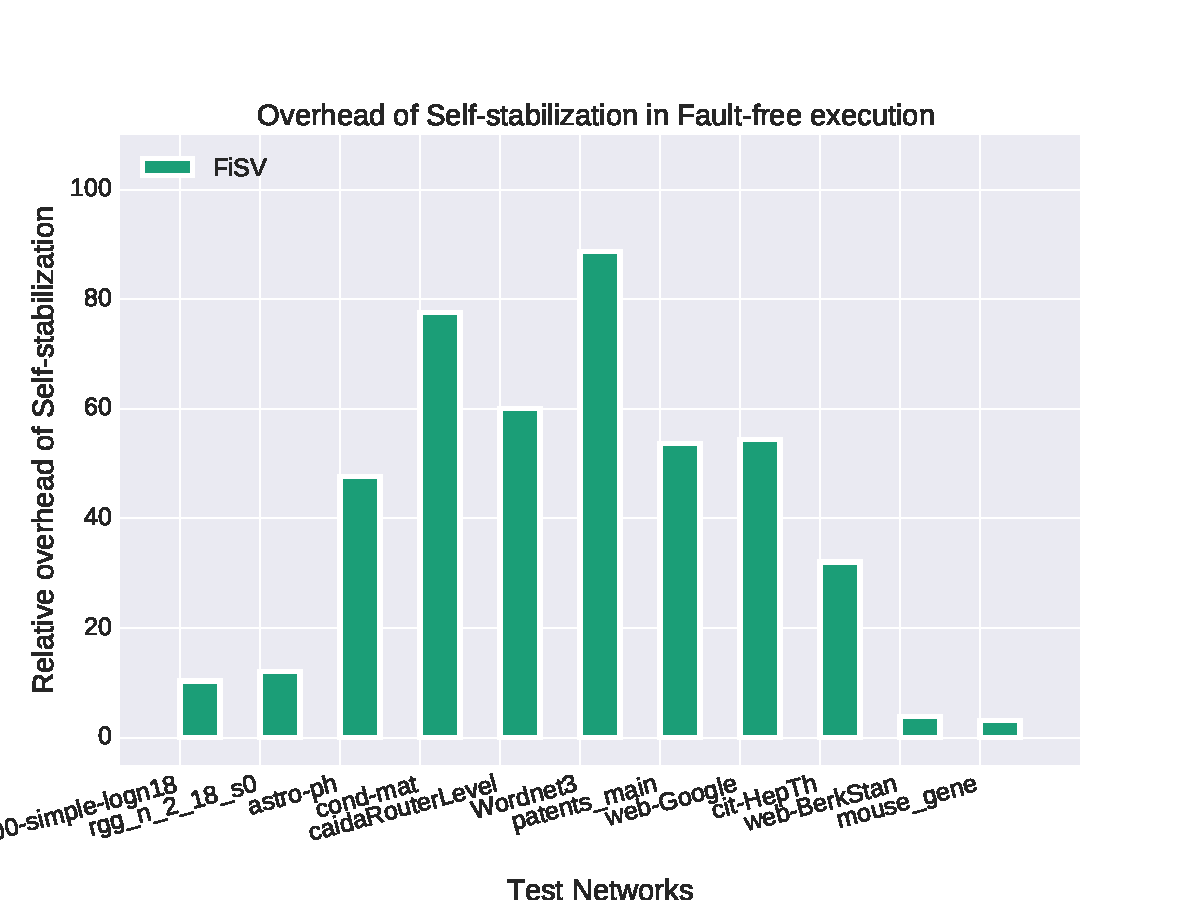
\includegraphics[width=0.95\columnwidth]{plots/timetest}\caption{Overhead of correction step for different networks}
\end{figure}

